\documentclass[11pt]{article}
\usepackage[a4paper, margin=2.54cm]{geometry}
\usepackage[utf8]{inputenc}
\usepackage[spanish, mexico]{babel}
\usepackage[spanish]{layout}
\usepackage[article]{ragged2e}
\usepackage{textcomp}
\usepackage{caption}
\usepackage{subcaption}
\usepackage{graphicx}
\usepackage{multirow}
\usepackage{amsmath}
\usepackage{amsfonts}
\usepackage{yhmath}
\usepackage{mathtools}
\usepackage{blkarray, bigstrut}

% ============================================================================
% ============================================================================
% ============================================================================

\title{
  TRABAJO PRÁCTICO FINAL\\
  \large Probabilidad y Estadística
}
\author{
  Farizano, Juan Ignacio \\
  \and
  Mellino, Natalia
}
\date{}

% ============================================================================
% ============================================================================
% ============================================================================

\begin{document}

\maketitle
\newpage

\tableofcontents
\newpage

% ============================================================================
% ============================================================================
% ============================================================================

\section{Ejercicio 1}

\subsection*{Apartado a)}

Para realizar la simulación utilizamos la siguiente función en R, donde recibe 
como parámetro la probabilidad $ p $ de que salga cara al tirar la moneda. Como
la moneda está equilibrada, en este caso la función tomará $ p = 0.5 $.

\begin{verbatim}
  simularCienTiradas <- function(P) {
    Sim <- sample(c("Cara", "Cruz"), 100, T, c(P, 1 - P))
    length(which(Sim == "Cara"))
  }
\end{verbatim}

Evaluando una vez esta función con parámetro $ p = 0.5 $ obtenemos:

\begin{verbatim}
  > simularCienTiradas(0.5)
  [1] 54
\end{verbatim}

En esta simulación el número de caras resultó ser 54.

% ============================================================================

\subsection*{Apartado b)}

Este apartado se puede resolver de dos formas distintas: una utilizando
la simulación y otra usando la teoría vista en clase. Para este apartado
interpretamos a $ X $ como $ X_{100} $.

\subsubsection*{Utilizando la simulación:}

Para hallar la $ P(X = 1) $ y la $ E(X) $ utilizamos el siguiente código, 
donde los argumentos recibidos $ N $ y $ P $ representan la cantidad de veces
que se simularán las cien tiradas (siendo N arbitrariamente grande) y P
es análoga al apartado a). En la función la variable \texttt{Acumulador}
es la suma de la cantidad de veces que salió cara en todas las simulaciones
y la variable \texttt{Uno} representa la cantidad de veces que una simulación
dió un numero de caras igual a uno.

\begin{verbatim}
  simularCienPorN <- function(N, P) {
    Acumulador <- 0
    Uno <- 0
    for (i in 1:N) {
      Sim <- simularCienTiradas(P)
      Acumulador <- Acumulador + Sim
      if (Sim == 1) {
        Uno <- Uno + 1
      }
    }
    c(Uno / N, Acumulador / N)
  }
\end{verbatim}

Cuando ejecutamos esta función, obtenemos los siguientes resultados:

\begin{verbatim}
  > simularCienPorN(1000000, 0.5)
  [1]  0.00000 49.98931
\end{verbatim}

Al intentar estimar los valores pedidos con la simulación, se obtuvo que
la $ P(X) = 1 $ es aproximadamente 0 (esto lo veremos al calcular el valor
de forma teórica, lo que sucede es que la probabilidad es tan chica que en
ninguna simulación sucede). Por otro lado, estimamos el valor de la esperanza
que se acerca a 50, que como veremos luego, éste es el valor exacto.

\subsubsection*{Utilizando la teoría:}

Para calcular $ P(X = 1) $ definimos una nueva variable aleatoria
$ Y $: número de caras obtenidas de un total de 100. Entonces, hallar
$ P(X = 1) $ es igual a hallar $ P(Y = 1) $, donde $ Y $ tiene una \textbf{Distribución
Binomial} de parámetros $ n = 100, \; p = 0.5 $, es decir, $ Y \sim B(100, 0.5) $.

\begin{align*}
  P(Y = 1) &= \binom{100}{1} \cdot 0.5^1 \cdot (1 - 0.5)^{100 - 1} \\
           &= 100 \cdot 0.5 \cdot 0.5^{99} \\
           &= 7.888609052 \cdot 10^{-29}
\end{align*}

Por lo tanto, $ P(X = 1) =  7.888609052 \cdot 10^{-29}$, que como podemos ver
es muy pequeña, y eso explica que no hayamos obtenido una buena estimación con
nuestra simulación.

Para hallar la esperanza de $ X $, hacemos:

\begin{equation*}
    E(X) = E(Y) = n \cdot p = 100 \cdot 0.5 = 50
\end{equation*}

Y así podemos afirmar que nuestra simulación pudo obtener una buena estimación
para $ E(X) $.

% ============================================================================

\subsection*{Apartado c)}

En este apartado, también se realizó de forma teórica y utilizando la simulación.

\subsubsection*{Utilizando la simulación}

Utilizamos el siguiente código:

\begin{verbatim}
  tresCaras <- function(N, P) {
    Acumulador <- 0
    for (i in 1:N) {
      Veces <- 0
      Tiradas <- 0
      while(Veces < 3) {
        Sim <- sample(c("Cara", "Cruz"), 1, T, c(P, 1 - P))
        if (Sim[1] == "Cara") {
          Veces <- Veces + 1
        }
        Tiradas <- Tiradas + 1
      }
      Acumulador <- Acumulador + Tiradas
    }
    Acumulador / N
  }
\end{verbatim}

y obtenemos el siguiente resultado:

\begin{verbatim}
  > buscarTres(1000000, 0.5)
  [1] 6.004526
\end{verbatim}

Entonces, se obtuvo que el número de veces a realizar el experimento hasta
obtener 3 caras es aproximadamente 6.

\subsubsection*{Utilizando la teoría}

Definimos una nueva variable aleatoria, $ Z $: número de veces que se realizó el
experimento hasta que salió cara por tercera vez. Esta variable aleatoria posee
una \textbf{distribución de Pascal} de parámetros $ r = 3 $ y $ p = 0.5 $. Lo que queremos
hallar nosotros entonces, es el número promedio de veces que se realizó el 
experimento hasta que salió cara por tercera vez, es decir, queremos hallar
$ E(Z) $, que viene dado por:

\begin{equation*}
  E(Z) = \frac{r}{p} = \frac{3}{0.5} = 6
\end{equation*}

Por lo tanto, el número promedio de veces que se deberá realizar el experimento hasta
que salga cara por tercera vez es 6.

% ============================================================================

\subsection*{Apartado d):}

El código dado en los apartados a) y b) ya permite que la moneda sea sesgada,
a continuación, realizamos la simulación parados valores diferentes de $ p $:
$ p = 0.01 $, $ p = 0.3 $ y $ p = 0.85 $

\begin{verbatim}
  simularCienPorN(1000000, 0.01)
  [1] 0.369727 1.000360

  > simularCienPorN(1000000, 0.3)
  [1]  0.00000 29.99997

  > simularCienPorN(1000000, 0.85)
  [1]  0.0000 84.9958
\end{verbatim}

De estas simulaciones, obtuvimos los siguientes resultados:

\begin{table}[h!]
  \begin{center}
    \begin{tabular}{| c | r | r |}
      \hline
      $ p $ & $ P(X = 1) $ & $ E(X) $ \\ \hline
      $ 0.01 $ & $ 0.3697 $ & $ 1.0003 $ \\ \hline
      $ 0.03 $ & $ 0.0000 $ & $ 29.9999 $ \\ \hline
      $ 0.85 $ & $ 0.0000 $ & $ 84.9958 $ \\ \hline 
    \end{tabular}
  \end{center}
\end{table}

% ============================================================================
% ============================================================================
% ============================================================================

\section{Ejercicio 2}

\subsection*{Apartado a)}
Para simular el proceso $ D_n $ utilizamos la siguiente función escrita en R

\begin{verbatim}
  trayectoriaD <- function(N, P) {
    Sim <- sample(c(1, 0), N, T, c(P, 1 - P))
    D <- vector()
    for (i in 1:N) {
      D[i] <- 2 * Sim[i] - 1
    }
    D
  }
\end{verbatim}

Para simular 10 pasos de una trayectoria de $ D_n $ (suponiendo que la moneda
está equilibrada) realizamos lo siguiente
\begin{verbatim}
  > trayectoriaD(10, 0.5)
  [1]  1  1 -1 -1  1  1  1  1 -1 -1
\end{verbatim}

% ============================================================================

\subsection*{Apartado b)}
Para simular el proceso $ S_n $ utilizamos la siguiente función escrita en R

\begin{verbatim}
  trayectoriaS <- function(N, P) {
    D <- trayectoriaD(N, P)
    S <- c(0)
    S[1] = 2 * D[1] -1
    for (i in 2:N) {
      S[i] <- S[i - 1] + D[i]
    }
    S
  }
\end{verbatim}

Y simulamos una trayectoria que graficamos

\begin{figure}[h!]
  \begin{center}
    \begin{subfigure}[b]{0.9\linewidth}
      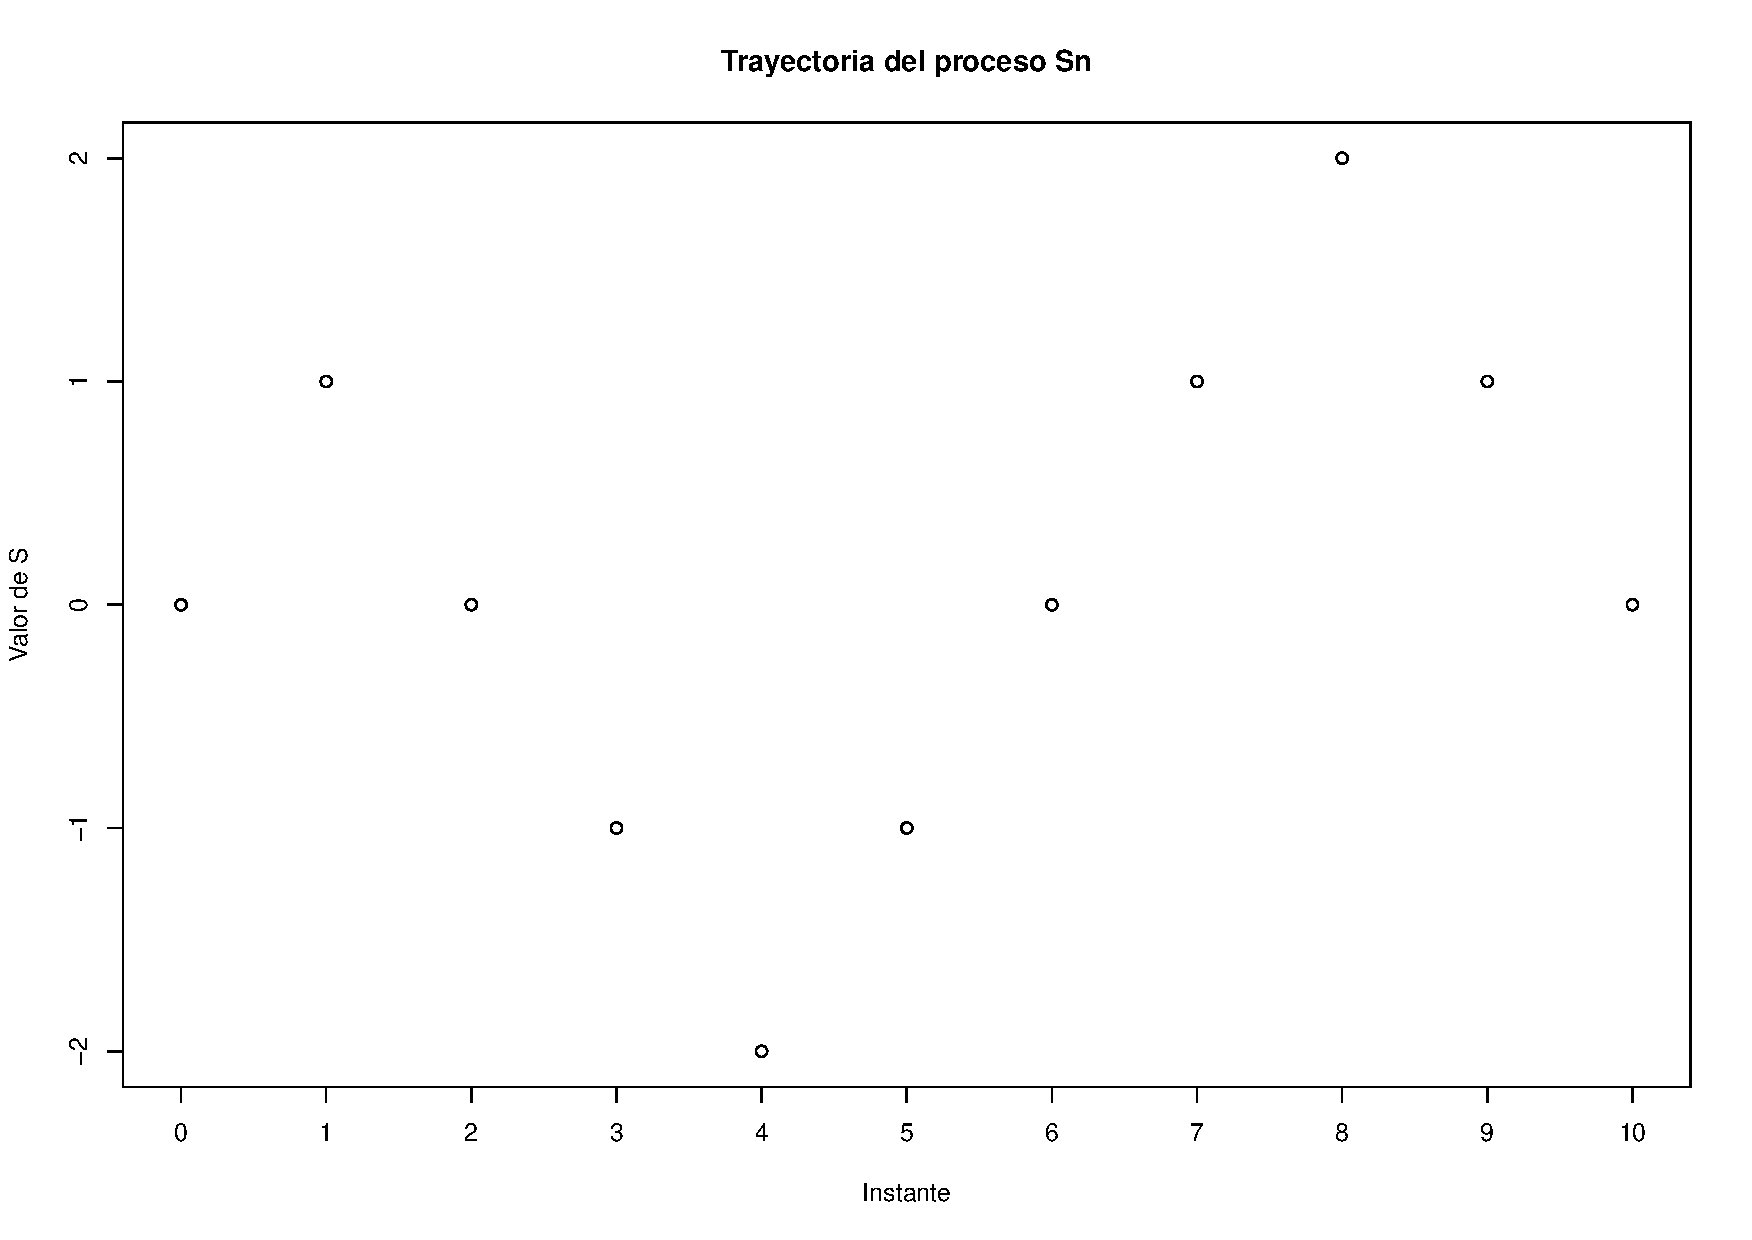
\includegraphics[width=\linewidth]{trayectoriaS.pdf}
    \end{subfigure}
  \end{center}
\end{figure}

% ============================================================================
% ============================================================================
% ============================================================================

\section{Ejercicio 3}

\subsection*{Apartado a)}

Para simular la trayectoria del jugador utilizamos el siguiente código en R:

\begin{verbatim}
  gamblersRuinTrayectoria <- function(P, K, S) {
    Pasos = 0
    Resultado = K
    Trayectoria = c(K)
    
    while (Resultado != 0 & Resultado != S) {
      Resultado = Resultado + sample(c(1, -1), 1, T, c(P, 1 - P))[1]
      Trayectoria = c(Trayectoria, Resultado)
      Pasos = Pasos + 1
    }
    
    plot(0:Pasos, Trayectoria, type = "p", xlab = "Instante", ylab ="Cantidad de dinero",
         main = "Trayectoria del jugador", ylim = c(0, S))
  }
\end{verbatim}

% ============================================================================

\subsection*{Apartado b)}

Utilizando el código escrito en a) con los valores $P = 0.6, \; K = 35, \; S = 100$ obtuvimos el
siguiente gráfico

\begin{figure}[h!]
  \begin{center}
    \begin{subfigure}[b]{0.9\linewidth}
      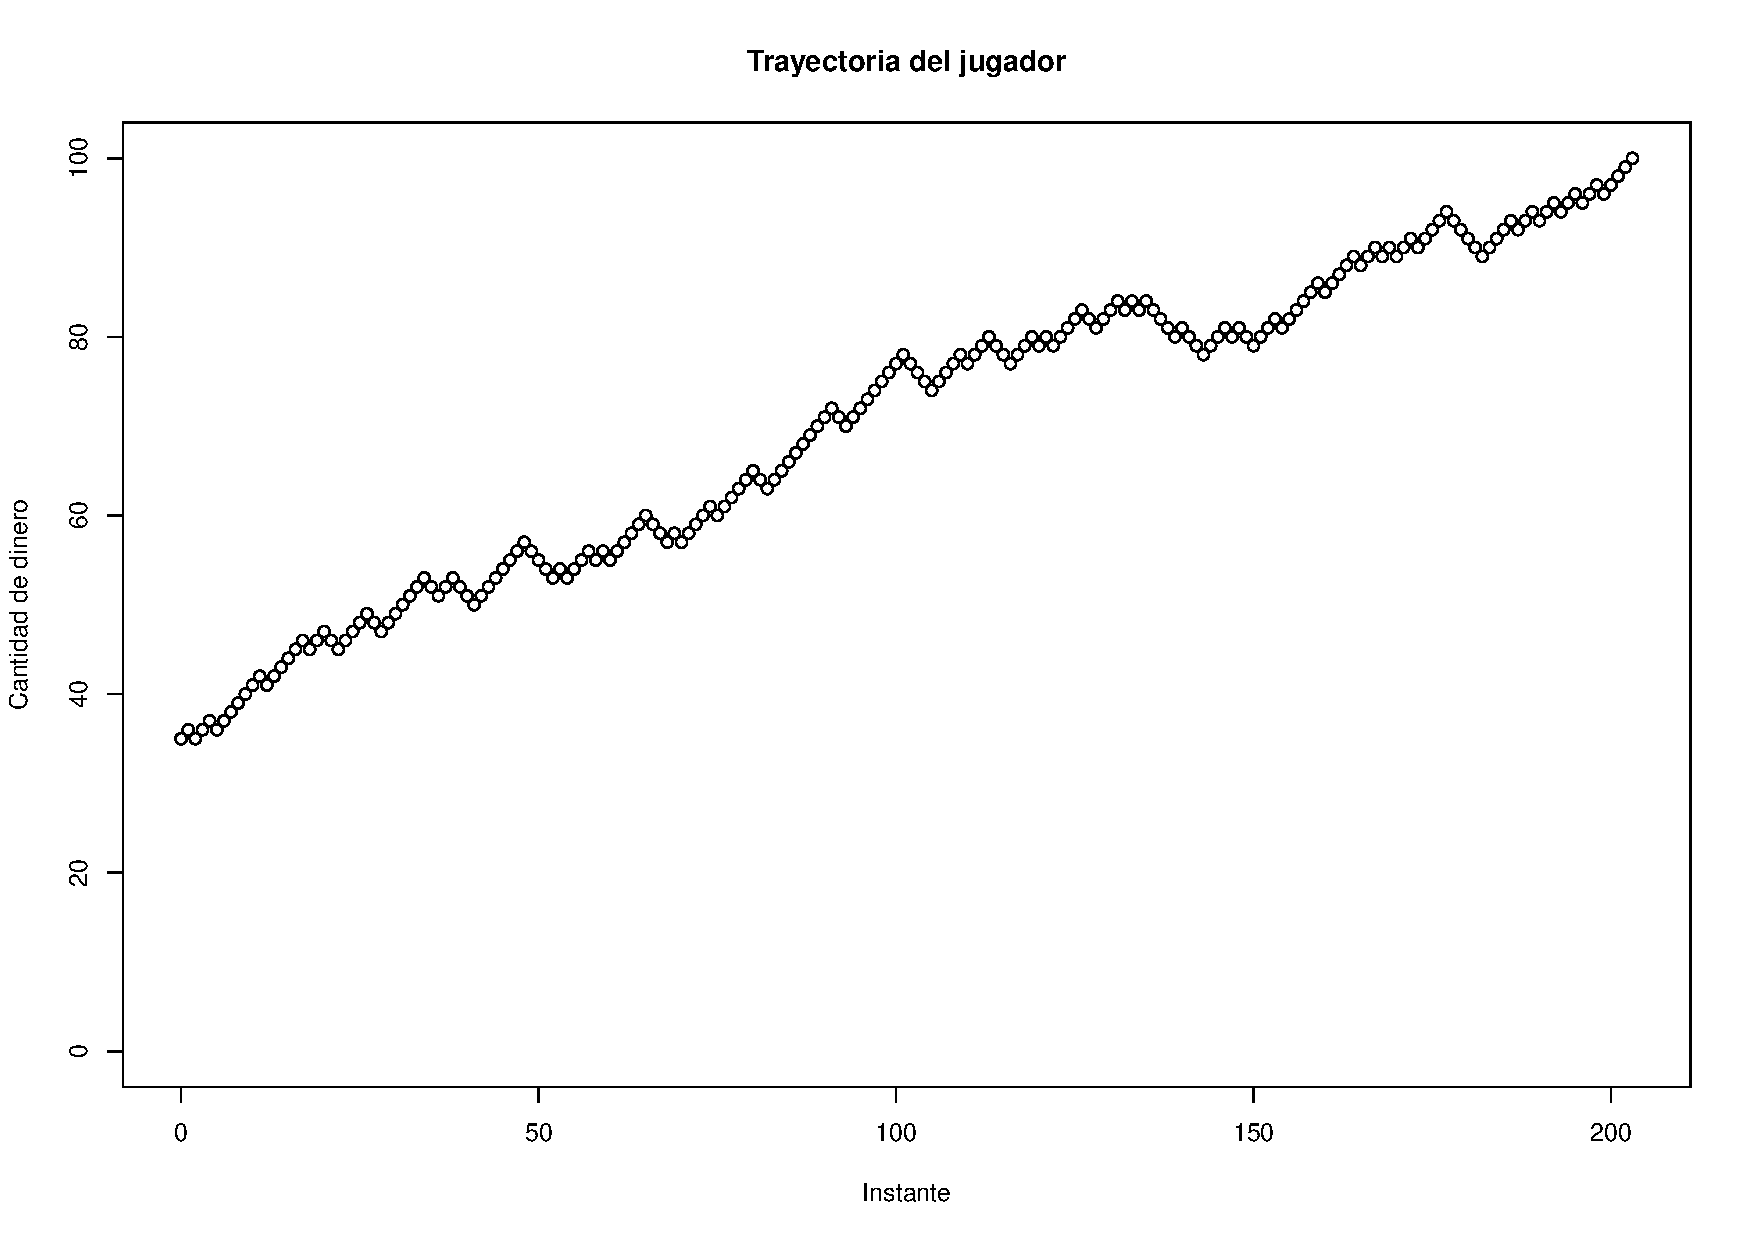
\includegraphics[width=\linewidth]{trayectoriaGamblers.pdf}
    \end{subfigure}
  \end{center}
\end{figure}

% ============================================================================

\subsection*{Apartado c):}

Resolvemos este apartado por simulación y luego comprobamos los resultados teóricamente.
Tomamos los valores: $ k = 3, \; S = 5,\; p = 0.65 $.

\subsubsection*{Simulación}

\begin{verbatim}
  calcularProbRuinaIter <- function(P, K, S, Simulaciones) {
    Arruinado <- 0
    Millonario <- 0
    for (i in 1:Simulaciones) {
      Resultado <- K
      Pasos <- 0

      while (Resultado != 0 & Resultado != S) {
        Resultado <- Resultado + sample(c(1, -1), 1, T, c(P, 1 - P))[1]
        Pasos <- Pasos + 1
      }
      if (Resultado == 0) {
        Arruinado <- Arruinado + 1
      }
    }
    Arruinado / Simulaciones
  }
\end{verbatim}

Y obtenemos como resultado:

\begin{verbatim}
  > calcularProbRuinaIter(0.65, 3, 5, 100000)
  [1] 0.11564
\end{verbatim}

\subsubsection*{Teórico}

Podemos modelar el problema como una Cadena de Markov estados: E = {0, 1, 2, 3, 4, 5},
donde la matriz de transición es:

\begin{equation*}
  P = 
  \begin{blockarray}{cccccccc}
     & & 0 & 1 & 2 & 3 & 4 & 5 \\
    \begin{block}{cc(cccccc)}
      0 & & 1    & 0    & 0    & 0    & 0    & 0 \\
      1 & & 0.35 & 0    & 0.65 & 0    & 0    & 0 \\
      2 & & 0    & 0.35 & 0    & 0.65 & 0    & 0 \\
      3 & & 0    & 0    & 0.35 & 0    & 0.65 & 0 \\
      4 & & 0    & 0    & 0    & 0.35 & 0    & 0.65 \\
      5 & & 0    & 0    & 0    & 0    & 0    & 1 \\
    \end{block}
  \end{blockarray}
\end{equation*}

Queremos estimar la probabilidad de ruinar del jugador, esto es hallar la $ F(k = 3, 0) $. 
Vimos en teoría que:

\begin{equation*}
  G(i, \; j) = F(i, \;, k) \forall k \in C_j
\end{equation*}

Sabemos que $ G = SB $, donde $ S = (I - Q)^{-1} $. Entonces procedemos a 
calcular las matrices correspondientes:

\begin{equation*}
  Q = 
  \begin{blockarray}{cccccc}
     & & 1 & 2 & 3 & 4 \\
    \begin{block}{cc(cccc)}
      1 & & 0    & 0.65 & 0    & 0    \\
      2 & & 0.35 & 0    & 0.65 & 0    \\
      3 & & 0    & 0.35 & 0    & 0.65 \\
      4 & & 0    & 0    & 0.35 & 0    \\
    \end{block}
  \end{blockarray}
\end{equation*}

\begin{equation*}
  B = 
  \begin{blockarray}{cccc}
     & & 0 & 5 \\
    \begin{block}{cc(cc)}
      1 & & 0.35 & 0   \\
      2 & & 0    & 0   \\
      3 & & 0    & 0   \\
      4 & & 0    & 0.65 \\
    \end{block}
  \end{blockarray}
\end{equation*}

\begin{equation*}
  S = 
  \begin{blockarray}{cccccc}
     & & 1 & 2 & 3 & 4 \\
    \begin{block}{cc(cccc)}
      1 & & 1.4759 & 1.3598 & 1.1441 & 0.7437 \\
      2 & & 0.7322 & 2.0920 & 1.7602 & 1.1441 \\
      3 & & 0.3317 & 0.9478 & 2.0920 & 1.3598 \\
      4 & & 0.1161 & 0.3317 & 0.7322 & 1.4759 \\
    \end{block}
  \end{blockarray}
\end{equation*}

\begin{equation*}
  G = 
  \begin{blockarray}{cccc}
     & & 0 & 5 \\
    \begin{block}{cc(cc)}
      1 & & 0.5165 & 0.4834 \\
      2 & & 0.2562 & 0.7437 \\
      3 & & 0.1161 & 0.8838 \\
      4 & & 0.0406 & 0.9593 \\
    \end{block}
  \end{blockarray}
\end{equation*}

Entonces, la probabilidad de ruina del jugador arracando con $ k = 3 $ es $ G(3, 0) \simeq 0.1161 $ (los resultados de la 
matriz $S$ y $G$ están redondeados a 4 cifras decimales). Observemos además que con la simulación
se obtuvo una buena aproximación a la probabilidad deseada.

\end{document}
